%
% assembly.tex
%
% Copyright (C) 2021 by SpaceLab.
%
% Flatsat Platform Documentation
%
% This work is licensed under the Creative Commons Attribution-ShareAlike 4.0
% International License. To view a copy of this license,
% visit http://creativecommons.org/licenses/by-sa/4.0/.
%

%
% \brief Board Assembly chapter.
%
% \author Gabriel Mariano Marcelino <gabriel.marcelino@spacelab.ufsc.br>
% \author Yan Castro de Azeredo <yan.azeredo@spacelab.ufsc.br>
%
% \institution Universidade Federal de Santa Catarina (UFSC)
%
% \version 0.1.0
%
% \date 2020/24/12
%

\chapter{Board Assembly}

The hardware project has the Bill of Material (BOM\nomenclature{\textbf{BOM}}{\textit{Bill Of Materials.}}) avalaible at its GitHub repository in excel spreeadsheets format. The PCB can be assembled by a Pick-and-place machine using the .txt file found on the hardware/fabrication folder if desired, fiducials labeled FD\# are placed to make this possible.

\section{FlatSat Stabillity Feet}

On the PCB there are labeled MEC1 to MEC12 mouting holes on the edges and in the middle of the board to be used for stabillity feet when the board is placed on top of a test bench.

\section{DNP Components}

There is only one Do Not Place (DNP\nomenclature{\textbf{DNP}}{\textit{Do Not Place.}}) component present in the USB to UART circuit, it is the labeled R4 pad with 0805 size (2012 metric) available for soldering the micro USB type B chassi to GND for Electromagnetic compatibility (EMC\nomenclature{\textbf{EMC}}{\textit{Electromagnetic Compatibility.}}) see \autoref{fig:R4-pad}. This can be done soldering a zero-Ohm resistor for a DC\nomenclature{\textbf{DC}}{\textit{Direct Current.}} path or capacitor for a high-frequency path between shield and signal ground, see Section 2.2.2 of the document \cite{ftdi-usb-hardware-guidelines} for more details.

\begin{figure}[!ht]
    \begin{center}
        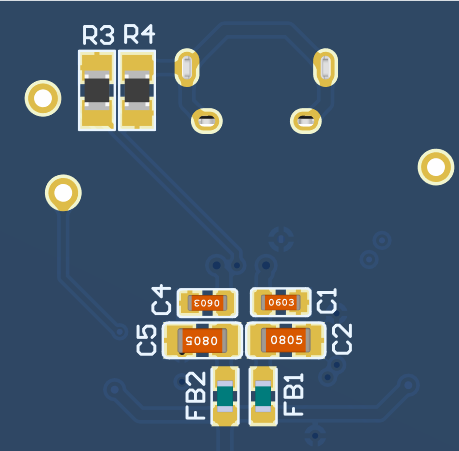
\includegraphics[width=0.5\textwidth]{figures/ft4232h_circuit_bottom.png}
        \caption{Bottom view of the UART to USB converter circuit.}
        \label{fig:R4-pad}
    \end{center}
\end{figure}

\section{Modules Mounting}

The PC-104 slots N$^{\circ}$2 to N$^{\circ}$7 are compatible for CubeSat PCB modules that are stacked in middle or the first on top. The slot N$^{\circ}$1 can only be used for the last module on this stack because of the inverted pinout. For the case of the SpaceLab's CubeSat stackup of the core modules, the last module of the stack is the EPS. For this case the EPS needs to be mounted up-side-down on slot N$^{\circ}$1 as can be seen on \autoref{fig:eps2-mouting}. For other modules any other PC-104 slots can be used, the OBDH\nomenclature{\textbf{OBDH}}{\textit{On-Board Data Handling.}} is showed mouted on \autoref{fig:obdh2-mouting}.

\begin{figure}[!ht]
    \begin{center}
        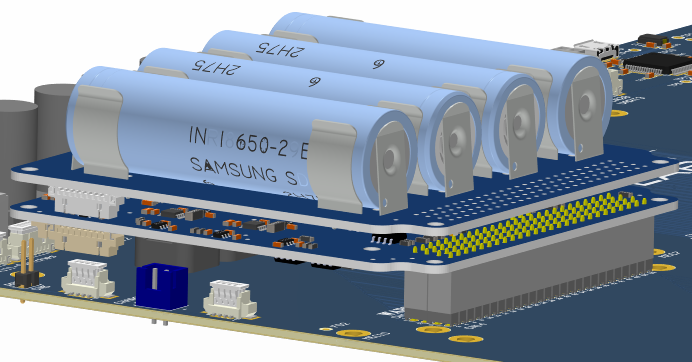
\includegraphics[width=0.8\textwidth]{figures/eps2_mouting.png}
        \caption{EPS mounted on N$^{\circ}$1 slot on a EDA tool.}
        \label{fig:eps2-mouting}
    \end{center}
\end{figure}

\begin{figure}[!ht]
    \begin{center}
        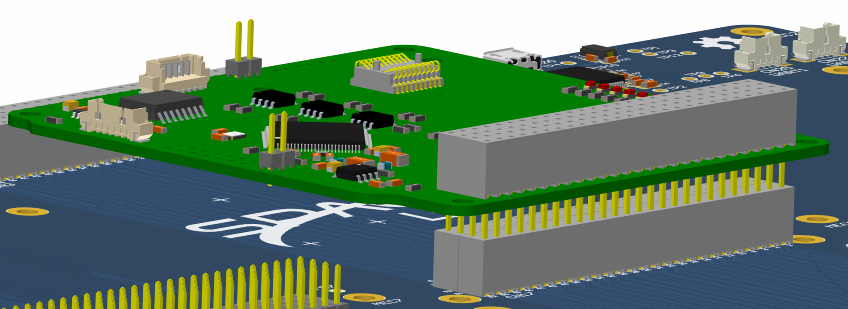
\includegraphics[width=0.8\textwidth]{figures/obdh2_mouting.png}
        \caption{OBDH mounted on N$^{\circ}$2 slot on a EDA tool.}
        \label{fig:obdh2-mouting}
    \end{center}
\end{figure}

\section{Antennas Connection}

Since the SMA connectors present on the board are on the right far side, modules placed in the opposite side may not be in reach for the connection. Because of this reason is recommended to use slots N$^{\circ}$1 and N$^{\circ}$4 for non antenna dependents PCBs.
